\chapter{BeagleBone Black Derivat}



\section{Übersicht}
Das BeagleBone Black-Derivat ist ein identischer Nachbau zum kostengünstigen Einplatinen-Computer BeagleBone Black. Es ist sowohl von der Funktion und dem Layout her praktisch identisch, kann aber, dank dieser Arbeit, selbst nach Abkündigung durch andere Hersteller immer noch von Variosystems hergestellt werden. Dies ermöglicht eine zeitliche Verfügbarkeitsgarantie und Unabhängigkeit von anderen Herstellern.


Da der BBB eine Open Source-Hardware ist, sind die eCAD-Pläne frei erhältlich. Die offiziellen Pläne sind allerdings mit dem eCAD-Tool mit dem Namen OrCAD erstellt worden \cite{bbbOrcad}. Diese Dateien sind aber nicht mit dem Altium Designer, dem eCAD-Tool welches in dieser Arbeit und bei Variosystems verwendet wird, kompatibel. Auf der Homepage von 'Element 14', einem offiziellen Distributor des originalen BBB, sind dennoch Pläne zu finden, welche mit dem Altium Designer erstellt wurden \cite{element14AltiumBBB}. Diese Pläne beziehen sich aber noch auf die 'Revision A5B', wobei 'Revision C' die aktuelle Revision ist. Alle Änderungen von Revision 'A5B' zur Revision 'C' wurden manuell in dieser Arbeit gemacht. Das Schema für das BBB-Derivat ist im Kapitel \ref{sec:anhang_schema_bbb_derivat} angehängt.



\section{Struktur des eCAD Projektes}

\subsection{Allgemeines}
Das elektrische Schema, das PCB Layout und auch die diversen Produktionsdateien, wie zum Beispiel die Gerber-Daten, wurden mit Altium Designer erzeugt. Zusätzlich wurde ein awk-Skript verwendet, um die Pick-and-Place-Datei richtig zu formatieren. Mehr dazu im Kapitel \ref{sec:awkSkript}.

\subsection{Aufbau des Schema}
Das Elektrische Schema ist, genau wie das Schema des originalen BBB, auf folgende 11 Top-Level-Blätter verteilt:

\begin{itemize}
\item P01: Titelblatt
\item P02: Power-Management
\item P03: Prozessor 1 und JTAG Header
\item P04: Prozessor 2/3, USB und Serial
\item P05: Prozessor 3/3
\item P06: LED, Bootup-Konfiguration und Taster
\item P07: DDR3 Arbeitsspeicher
\item P08: eMMC Festspeicher
\item P09: Ethernet
\item P10: HDMI
\item P11: Stiftleisten, $\mu$SD und EEPROM
\end{itemize}

Im Folgenden wird nur noch auf die Seitennummer des Schema (P01...P11) verwiesen, und nicht mehr auf den Namen. 


\subsection{Bauteile und Bauteilbibliotheken}
Alle verwendeten Bauteile haben einen sogenannten 'Life Supplier Link'. Dieser Link verweist direkt auf die Datenbanken der Distributoren. Durch diesen Link kann die Stückliste automatisch erstellt werden. Aus der Stückliste ist direkt ersichtlich, ob das Bauteil beim jeweiligen Distributor vorrätig ist, und wie hoch der Kaufpreis es in der benötigten Menge aktuell ist.

Wenn möglich, wurde Digi-Key als Distributor gewählt. Wenn das Bauteil bei Digi-Key nicht erhältlich oder nicht vorrätig war, wurde auf Mouser oder Arrow ausgewichen. Bei Arrow funktionierte der Life-Link allerdings nicht. Aus diesem Grund wurde die Stückliste bei allen Bauteilen von Arrow manuell ergänzt. In der Stückliste sind diese manuellen Ergänzungen gelb hinterlegt.

Widerstände und Kondensatoren, welche auch in der Bauteilbibliothek von Variosystems vorhanden sind, haben einen Parameter mit dem Namen 'VS Part Number'. In diesem Parameter ist die Artikelnummer von Variosystems hinterlegt, die dem entsprechenden Standardbauteil von Variosystems entspricht.

\subsection{Output Files}
Als 'Output Files' werden im Altium Designer alle Dateien bezeichnet, welche aus dem elektrischen Schema oder dem PCB Layout erzeugt werden. Diese Dateien werden in einem 'Output Job' (BBB\_Derivat.OutJob) definiert. Dieser 'Output Job' enthält folgende Container, welche die entsprechenden Dateien erzeugt:

\begin{itemize}
\item Assembly: Erzeugt PDFs, welche beim Bestücken des PCBs hilfreich sein können.
	\begin{itemize}
	\item ASSEMBLY\_Print.pdf: Ein Plan, der bei der Positionierung der Bauteile auf dem PCB hilft
	\end{itemize}
\item Production Data: Erzeugt alle Dateien, welche für die Herstellung und Bestückung des PCBs notwendig sind.
	\begin{itemize}
	\item Pick And Place Files: Dateien für die Pick-and-Place Maschine. Mehr dazu im Kapitel \ref{sec:awkSkript}.
	\item Gerber Files: Die Gerber Daten werden für die Produktion des PCBs benötigt.
	\item NC Drill Files: Plan für die Bohrungen.
	\item Bill of Materials: Stückliste. Diese wird automatisch mit den aktuellen Informationen aus den 'Life Supplier Link' ergänzt.
	\end{itemize}
\end{itemize}

%TODO evt ergänzungen

\subsection{Pick and Place: awk Skript}\label{sec:awkSkript}
'awk' ist eine Skriptsprache, die auf einfache Weise erlaubt, strukturierten Text zu bearbeiten.

Der Altium Designer erzeugt eine Datei mit den Informationen für die Pick and Place Maschine. In dieser Datei ist unter Anderem der Designator, die Position und der Drehwinkel des Bauteils gespeichert.

Die Pick and Place Maschine von Variosystems benötigt aber je für die obere und die untere Lage eine separate Datei. Des Weiteren sollten die Artikelnummer von Variosystems für die entsprechenden Standardbauteile hinzugefügt und unnötige Informationen entfernt werden. Diese Aufgabe wurde mit dem awk-Skript 'Pick-n-Place-Separator.awk' (siehe Anhang Kapitel XXX) automatisiert.
%TODO auf angehängtes Skript XXX verweisen

Bei der Bestückung bei Variosystems hat sich aber gezeigt, dass diese Dateien gar nicht verwendet wurden. Die Technische Abteilung von Variosystems hat die Pick and Place Datei selber aus der PCB ASCII Datei (*.PcbDoc) erstellt. Das PCB wird normalerweise in einem binären Format gespeichert. Um das PCB-Layout als eine ASCII-Datei zu speichern, muss diese mit der Funktion 'Speichern unter...' speziell erzeugt werden.

\section{Upgrade auf Revision C}\label{sec:upgrade_rev_c}
Im Folgenden werden alle Änderungen aufgelistet, welche gemacht wurden, um die Pläne von 'Element 14' an die 'Revision C' anzupassen. Die zusätzlichen Bauteile wurden auf dem PCB an den gleichen Position platziert, wie auf dem originalen BBB.

\begin{itemize}
\item A5C: 
%Diese Änderungen wurden wegen Produktionsfehler, verursacht von Unterschieden in den Widerständen, gemacht.
	\begin{itemize}
	\item R46, R47 und R48 auf 0$\Omega$ geändert.
	\item R45 auf 22$\Omega$ geändert.	
	\end{itemize}
\item A6:
	\begin{itemize}
	\item Der 'Enable' Eingang des VDD\_3V3B Spannungsregler (U4) ist neu mit VDD\_3V3A verbunden.
	\item AND-Gate (U16) hinzugefügt.	
	\item Optionaler 0$\Omega$ Widerstand (R29) hinzugefügt.	
	\end{itemize}
\item A6A:
	\begin{itemize}
	\item Optionaler 0$\Omega$ Widerstand (R30) hinzugefügt.
	\item C106 auf 1$\mu$F geändert.
	\item C24 auf 2.2$\mu$F geändert.
	\item R8 auf 'Bestücken' und R9 auf 'Nicht bestücken' gesetzt.
	\end{itemize}
\item B:
	\begin{itemize}
	\item Der Prozessor (U5) ausgewechselt. Neue Modellnummer: AM3358BZCZ100.	
	\end{itemize}
\item C:
	\begin{itemize}
	\item Den eMMC Speicher (U13) von 2GB auf 4GB erhöht.
	\end{itemize}
\end{itemize}



\section{Elektrisches Schema}
Die Hardware und die Funktion des BBB, und somit auch des BBB-Derivates, wird im 'System Reference Manual (SRM) \cite{adafruitSRM} ausgiebig beschrieben. Aus diesem Grund wird im Folgenden nur auf Aspekte eingegangen, die im Zusammenhang mit dem ComCape interessant sind, oder nicht im SRM erwähnt werden.


\subsection{Power-Management}
Der Power-Management-IC TPS65217\textit{CRSLR} (U2) stellt zusammen mit dem TL5209 (U4) die verschiedenen Spannungspegel zur Verfügung. Der TPS65217\textit{CRSLR} (U2) ist dabei speziell auf den verwendeten Prozessor AM3358BZCZ100 (U5) und den DDR3 Arbeitsspeicher abgestimmt.

Das BBB-Derivat kann über die Mini-USB-Buchse oder mit einem separaten 5V-Netzteil betrieben werden. Wird es allerdings zusammen mit dem ComCape genutzt, ist es unbedingt notwendig, dass ein Netzteil mit mindestens 2A verwendet wird. Die Spannungsversorgung nur über USB ist dann nicht ausreichend.


Die verschiedenen Versorgungsspannungen sind in Tabelle \ref{tab:versorgungsspannungen} zusammengefasst. Im SRM\cite{adafruitSRM} werden diese noch genauer beschrieben.

\begin{table}

    \begin{tabular}{ | l | l | l | p{7cm} |}
    \hline
    \textbf{Name}		& \textbf{Spannung} 	& \textbf{Max. Strom} 	& \textbf{Beschreibung} \\ \hline
    
    VRTC		& 1.8V		& 250mA	 		& Wird beim Powerup als erstes aktiviert. Speist die IO Spannung des Power-Management-IC und die Echtzeituhr des Prozessors.\\ \hline    
    
    VDD\_3V3A 	& 3.3V 		& 400mA 		&  3.3V Stromversorgung für den Prozessor. Da die Stromstärke aber nicht für die Peripherie ausreicht, ist ein zusätzlicher, diskreter Spannungsregler verbaut. Siehe 3V3B.\\ \hline
    
    VDD\_3V3B	& 3.3V 		& 500mA 		& 3.3V Stromversorgung für Peripherie. Dazu gehören: JTAG, UART0, eMMC, Ethernet, HDMI und die $\mu$SD. Mit dem Pin \textit{AI7} des Prozessors (U5) kann diese Spannung gemessen werden. Diese Spannung wird über die Stiftleiste geführt, und kann für die Signalpegelwandler verwendet werden.\\ \hline
    
    VDD\_5V		& 5V 		& 2'000mA 		& 5V Spannung direkt vom externen Netzgerät. Die maximale Stromstärke wird auch vom verwendeten Netzgerät begrenzt. Dabei darf nicht vergessen werden, dass der BBB indirekt ebenfalls über das externe Netzgerät gespeist wird, und dieses belastet. Diese Spannung ist nicht präsent, wenn der BBB nur über USB und nicht mit einem externen Netzgerät gespeist wir. Ein einzelner Pin darf maximal mit 1'000mA belastet werden. Diese Spannung wird über zwei Pins zum Cape geführt.\\ \hline
    
    SYS\_5V		& 5V 		& 500mA 		& Diese 5V werden vom Power-Management IC von der USB-Spannung oder vom externen Netzgerät generiert. Diese Spannung wird vom Power-Management-IC selbst verwendet.\\ \hline
    
    VDD\_1V8	& 1.8V 		& 400mA 		& Exklusiv für den Prozessor und den HDMI Framer.\\ \hline
    
    VDD\_CORE	& 1.1V 		& 1'200mA 		& Exklusiv für den Prozessor.\\ \hline
    
    VDD\_MPU	& 1.1V 		& 1'200mA 		& Exklusiv für den Prozessor.\\ \hline
    
    VDD\_CORE	& 1.5V 		& 1'200mA 		& Exklusiv für den DDR3. Kann für DDR3L auf 1.35V gesenkt werden.\\ \hline
    
    
    \end{tabular}
    \caption{Versorgungsspannungen des BBB}
    \label{tab:versorgungsspannungen}

\end{table}



\subsection{Spannungspegel für die digitale Kommunikation}
Die digitalen IOs des Prozessors können grundsätzlich mit 1.8V oder mit 3.3V gespeist werden. Auf dem BBB-Derivat werden sie mit 3.3V betrieben. Aus diesem Grund haben die digitalen IOs einen TTL-Spannungspegel von 3.3V. Dieser Spannungspegel wird von der $\mu$SD-Karte benötigt.

\subsection{Power-Up-Sequence}
Damit der BBB nicht beschädigt wird, müssen die verschiedenen Spannungsversorgungen in der richtigen Reihenfolge gestartet werden. Dies wird bereits vom Power-Management-IC übernommen.

Im SRM \cite{adafruitSRM} auf Seite 113 wird darauf hingewiesen, dass keine Spannungen an die IO-Pins des Prozessors angelegt werden, bevor die \textit{VDD\_3V3B} Spannungsversorgung gestartet wird. Das BLE-Modul wird über diese Spannungsversorgung gespeist. So ist es nicht möglich, das BLE-Modul eine Spannung anlegt, bevor \textit{VDD\_3V3B} gestartet wird.
Das WLAN-Modul und das GSM-Modul sind über einen Spannungspegelwandler (\textit{TXS0108E}) mit dem Prozessor verbunden. Die 3.3V-Seite des Pegelwandlers, welche mit dem Prozessor verbunden ist, wird ebenfalls über die \textit{VDD\_3V3B} Spannungsversorgung gespeist. So wird verhindert, dass beim Prozessor eine Spannung anliegt, bevor \textit{VDD\_3V3B} gestartet ist.

Auch \textit{VDD\_5V} darf nicht belastet werden, bevor \textit{VDD\_3V3B} gestartet ist. Dies ist aber kein Problem, da \textit{VDD\_5V} auf dem ComCape nicht verwendet wird.

\subsection{Optionale Komponenten}
Für die Kernfunktion des BBB, also booten und ausführen des Betriebssystems, sind nicht alle verbauten Bauteile notwendig. Für bestimmte Funktionen werden diese zusätzlichen Bauteile aber gebraucht. Im Schema des BBB-Derivats sind diese Bauteile mit einer grünen Strich-Punkt-Linie umrandet, und mit grüner Schrift betitelt. Alle anderen Komponenten sind für das Ausführen eines Betriebssystems notwendig. Wenn eine Funktion auf dem BBB-Derivat nicht benötigt wird, kann auf alle Bauteile in der Umrahmung verzichtet werden. Diese optionalen Funktionen werden in der Tabelle \ref{tab:optionaleFunktionen} aufgelistet.


\begin{table}
    \begin{tabular}{ | p{2.5cm} | l | p{9.5cm} |}
    \hline
    \textbf{Funktion}		& \textbf{Blatt} 	& \textbf{Funktion} \\ \hline
    
    Clock HDMI Framer		& P03		& Dieser Clock wird nur für die HDMI-Schnittstelle benötigt (P10 'HDMI').\\ \hline   
    
    Clcok McASP				& P03		& Dieser Clock wird benötigt, wenn die McASP Schnittstelle verwendet wird.\\ \hline   
    
    JTAG Schnittstelle		& P03		& Bietet einen Header für die JTAG-Verbindung zum Prozessor. Diese Schnittstelle wird auch auf dem originalen BBB nicht bestückt.\\ \hline  
    
    UART 0 Debugschnittstelle	& P04		& Eine elektrisch isolierte UART Verbindung (UART0), auf die über die Stiftleisten J1 zugegriffen werden kann. Diese Verbindung kann auch als Debugschnittstelle verwendet werden. \\ \hline      
    
    USB Host				& P04		& USB Host Funktionalität des BBB.\\ \hline    
    
    USB PC Connector		& P04		& Über die USB-Mini-Buchse kann der BBB mit einem PC verbunden werden. Durch diese Verbindung kann der BBB mit Spannung versorgt werden. Zusätzlich kann über diese Verbindung von einem separatem PC auf die Entwicklungsumgebung und die Daten auf dem BBB zugegriffen werden.\\ \hline    
    
    User LED				& P06		& LEDs, die den Status des BBB anzeigen, und auch individuell Programmiert werden können.\\ \hline  
    
    eMMC					& P08		& Dies ist der 4GB grosse Festspeicher des BBB. Das Betriebssystem kann allerdings auch direkt von der $\mu$SD gebootet werden. Das System läuft aber deutlich schneller, wenn es vom eMMC gestartet wird. \\ \hline 
    
    Ethernet				& P09		& Ethernet-Verbindung inklusive PHY und Buchse. Der MAC ist im Prozessor integriert.\\ \hline    
    
    HDMI					& P10		& Der HDMI-Framer wandelt das LCD-Signal vom BBB in ein HDMI-kompatibles Signal um, welches von einem normalen, HDMI-fähigen Monitor wiedergegeben werden kann. Dies funktioniert aber nur, wenn die LCD-Pins des BBB nicht für einen LCD oder andere Funktionen verwendet werden. Zusätzlich wird noch das Taktsignal für den HDMI benötigt (siehe P03 'Clock HDMI Framer'). \\ \hline   
    
    LCD or HDMI				& P10		& Diese Kondensatoren werden nur benötigt, wenn entweder ein externer LCD angeschlossen wird, oder wenn der HDMI Ausgang benutzt wird.\\ \hline 
    
    Expansion Header& P11		& Über die beiden Stiftleisten können die diversen Capes, unter anderem auch das ComCape, verbunden werden.\\ \hline 

    \end{tabular}
	\caption{Optionale Funktionen des BBB}
	\label{tab:optionaleFunktionen}
\end{table}


\subsection{$\mu$SD}
Das Betriebssystem kann wahlweise von der $\mu$SD oder vom eMMC aus gebootet werden. Eine $\mu$SD Karte ist eine „Mikro-Secure-Digital Flash Speicherkarte“ welche auch in vielen Smartphones als Erweiterung für den internen Speicher dient. Um den fabrikneuen und unbeschriebenen eMMC mit einem bootfähigen Betriebssystem zu beschreiben, wird eine $\mu$SD mit einem speziellen Image benötigt. Auf dieses Thema wird im Softwareteil der Dokumentation im Kapitel [XXX] noch weiter eingegangen.
%TODO Kapitel EGEMEN


\subsection{DDR3L RAM}
Der DDR3L SDRAM ist ein RAM, der mit einer Spannungsversorgung von 1.35V betrieben werden kann. Im BBB-Derivat, wie auch beim originalen BBB, wird er aber im Rückwärtskompatibilitätsmodus  mit 1.5V betrieben. Dies wurde so gelöst, damit am originalen BBB Design möglichst wenig verändert werden musste.


\subsection{I$^2$C EEPROM}
Auf dem BBB befindet sich ein EEPROM, der über I$^2$C angesprochen werden kann. Für das Booten des Betriebssystems sind bestimmte Informationen auf dem EEPROM notwendig. Ohne diese Informationen startet der BBB nicht.

Zum Programmieren der 5 EEPROMS für die 5 Prototypen wurde ein Arduino-Klon mit dem Namen 'MINI-AT Board' verwendet. Zusätzlich wurde ein SchmartBoard\textsuperscript{TM} verwendet. Auf dem SchmartBoard\textsuperscript{TM} sind die beiden Pull-Up Widerstände, welche für den I$^2$C benötigt werden, aufgelötet. Zusätzlich bietet es Platz um die EEPROMS aufzulöten. Ein SchmartBoard\textsuperscript{TM} ist ein Prototypen-PCB, welches speziell dafür ausgelegt ist, um SMT Bauteile von Hand aufzulöten. In Abbildung XXX ist das 'MINI-AT Board' mit dem SchmartBoard\textsuperscript{TM} zu sehen. Abbildung YYY zeigt die elektrische Verdrahtung des Arduino-Klons um ein EEPROM zu programmieren.

Wie der EEPROM genau programmiert wurde, wird im Softwareteil im Kapitel XXX beschrieben.

%TODO Verweis auf SW
%TODO Bild Audrino + Verweis XXX
%TODO Bild El Schema Audrino EEPROM YYY


\subsection{Belegung der Pinheader}
Die verwendete Pinbelegung der Erweiterungs-Stiftleisten P8 und P9 ist im Anhang \ref{sec:anhang_pinbelegung} dokumentiert. Alternative Pinbelegungen sind im 'System Reference Manual'\cite{adafruitSRM}  des BBB dokumentiert.




\section{Aufbau des PCB}\label{aufbauPCB}
Für digitale Hochgeschwindigkeitskommunikation spielt die Wellenimpedanz der Leiterbahnen eine grosse Rolle. Die Impedanz wird durch den Lagenaufbau des PCBs, aber auch durch die Breite der Leiterbahnen definiert. Man unterscheidet dabei zwischen 'Single-Ended' und 'Differential Pair'. Bei einem 'Differential Pair' werden zwei Leiterbahnen benötigt, die in einem definiertem Abstand parallel zueinander geführt werden.

In diesem Layout kommen die Impedanzen Single '50$\Omega$', 'Differential 90$\Omega$' und 'Differential 100$\Omega$' vor. Wenn das Layout des PCB mit dem Altium Designer geöffnet wird, sind die Leiterbahnen der verschiedenen Impedanzen in den Netklassen 'Single\_50', 'Diff\_90' und 'Diff\_100' sortiert.

Die PCBs wurden speziell mit Impedanzkontrolle bestellt, damit eine definierte Impedanz gewährleistet werden konnte. Auf Anfrage hat der Hersteller, Multi Circuit Borads, eine Tabelle mit dem Lagenaufbau und den benötigten Leiterbahnbreiten für die gewünschten Impedanzen (siehe Abbildung \ref{LagenaufbauBB}) geschickt.

In Abbildung \ref{LagenaufbauBB} ist ebenfalls zu sehen, dass die benötigte Leiterbahnbreite für eine bestimmte Impedanz für die Innenlagen anders ist, als für die Aussenlagen. Alle Leiterbahnen, welche eine vordefinierte Impedanz und somit auch eine genau definierte Breite benötigen, wurden auf dem PCB Layout des BBB-Derivats angepasst.

Das PCB des BBB hat 6 Lagen. \textit{TOP} und \textit{BOTTOM} sind die beiden Aussenlagen. Die zweite Lage, \textit{L2}, ist komplett gefüllt mit einer GND-Fläche. Die beiden innersten Lagen, \textit{L3} und \textit{L4}, werden für Leiterbahnen verwendet. Die 5. Lage, \textit{L5}, ist für die Spannungsversorgung reserviert.


\begin{figure}[!ht]
\centering
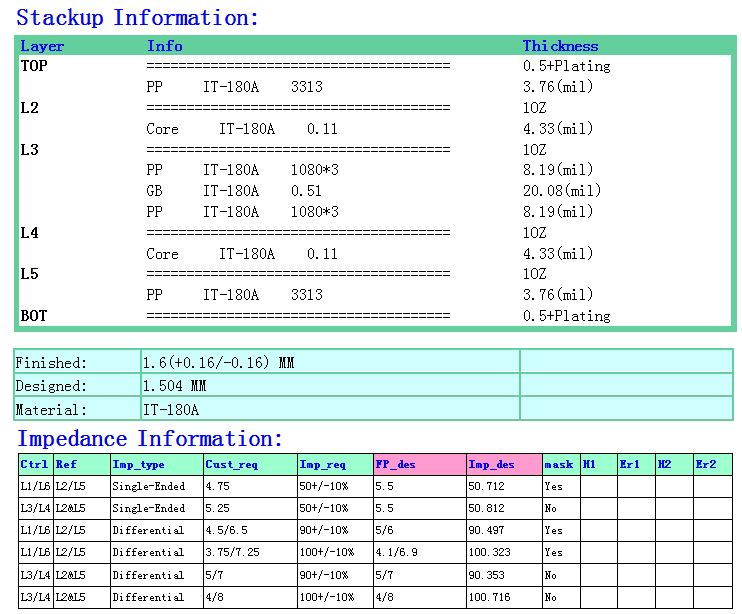
\includegraphics[angle=0,width=14cm]{images/LagenaufbauBB.jpg}
\caption{Lagenaufbau und Impedanzen des BBB}
\label{LagenaufbauBB}
\end{figure}


\section{Layout des PCB}

\subsection{Änderungen}
Am Layout des PCB, welches von der 'Element 14'-Homepage stammt, wurden folgende Änderungen vorgenommen:

%TODO detailierter; evt. Bilder
\begin{itemize}
\item Die Leiterbahnbreiten für die kontrollierten Impedanzen wurden entsprechend angepasst
\item Alle Änderungen für das Upgrade auf die Revision C (siehe \ref{sec:upgrade_rev_c}).
\item Der obere und unter Beschriftungsdruck wurde so angeordnet, dass die Designatoren gut sortiert und lesbar sind
\end{itemize}


\subsection{Kritische Stellen des Layouts}
Bei digitalen Hochgeschwindigkeitsübertragungen ist die Signalintegrität von grosser Bedeutung. Die Signalintegrität beschreibt, wie gut das gesendete Signal des Senders mit dem Signal übereinstimmt, welches der Empfänger am anderen Ende der Leitung empfängt. Wenn die Signalintegrität zu klein ist, kann es zu Datenverlusten führen. Dieser Datenverlust kann dazu führen, dass die Datenverbindung nicht mehr brauchbar ist. Wenn z.B. die Signalintegrität der Verbindung zwischen dem Prozessor und dem RAM zu schlecht ist, kann der Prozessor den RAM gar nicht mehr nutzen. Da der BBB ohne RAM nicht lauffähig ist, muss dies unbedingt verhindert werden.

Für eine gute Signalintegrität muss unter anderem die Impedanz der Leiterbahnen stimmen. Dieses Thema wurde bereits im Kapitel \ref{aufbauPCB} diskutiert. Zusätzlich müssen alle Leiterbahnen gleich lang sein, damit alle Signale gleichzeitig ankommen. Elektromagnetische Störungen von aussen können die Signalintegrität ebenfalls beeinflussen.

In Abbildung \ref{kritischeStellenBBB} sind alle Leiterbahnen, bei denen die Signalintegrität ein kritischer Faktor sein könnte, rot eingerahmt. Ohne detailliertes Wissen über digitale Signalintegrität, sollte das PCB Layout in diesem Bereich nicht geändert werden.

\begin{figure}[!ht]
\centering
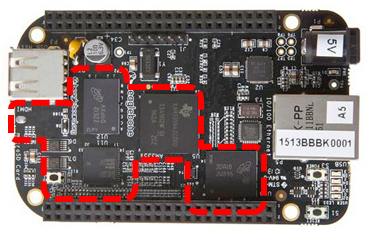
\includegraphics[angle=0,height=5cm]{images/BBB_kritische_stellen.png}
\caption{Kritische Stellen des BBB}
\label{kritischeStellenBBB}
\end{figure}




\section{Produktion der Prototypen}


\subsection{Vorgehen}
Die PCBs wurden von der Firma 'multi-cb' gefertigt. Die fertigen PCB sind dann beim Industriepartner Variosystems bestückt worden. Es wurden 10 PCBs bestellt, fünf davon sind bestückt worden.

Bei einer Bestückung durchläuft das PCB mehrere Stationen. Zuerst wird die Lötpaste auf das PCB aufgetragen. Anschliessend werden alle Bauteile durch einen Pick-and-Place-Roboter auf dem PCB platziert. In einem Reflow-Ofen wird dann das ganze PCB inklusive Bauteile und Lötpaste erhitzt, so dass die Bauteile endgültig mit dem PCB verlötet werden. Diese Schritte werden einmal für die Oberseite und einmal für die Unterseite ausgeführt. Mit einem Röntgengerät können dann auch die Lötstellen unter einem Bauteil kontrolliert werden.

Aufgrund von Firmenrichtlinen konnten bei der Bestückung leider keine Fotos von der Produktionsstrasse geschossen werden.


\subsection{Lötpaste}
Bei der ersten Station der Produktion wurde zuerst eine Lötpastenmaske aus dünnem Stahlblech genau über das PCB gelegt. Die Ausschnitte des Bleches entsprechen dem Layer \textit{Top Paste} und \textit{Bottom Paste} im PCB Dokument. Über diese Maske wurde feinkörnige, bleifreie Lötpaste gestrichen, die bei den Aussparungen der Maske auf dem PCB haften bleibt.

Der Nutzenrand des PCBs (siehe Abbildung XXX) war hier von grossem Vorteil. Dank diesem Rand konnte das PCB problemlos auf dem Förderband fixiert werden, ohne dass Lötstellen verdeckt werden. Nachdem die Lötpaste aufgetragen wurde, wurde das PCB auf einem Förderband zum Pick and Place Roboter transportiert.
%TODO Foto PC mit Nutzenrand


\subsection{Pick-and-Place-Roboter}
Im Pick-and-Place-Roboter wurden alle SMT Bauteile bestückt. Der Roboter platziert dabei alle SMT Bauteile auf dem PCB, durch die Lötpaste schwach auf dem PCB haften.

Das Einrichten der Maschine war ein sehr grosser Initialaufwand. Nachdem der Roboter aber richtig eingestellt wurde, ging das Bestücken zügig und ohne grössere Probleme voran. Aus diesem Grund ist diese Maschine nur bei grossen Stückzahlen effizient. 

Der Roboter hat leider immer wieder Bauteile verloren, die mühsam in der Maschine gesucht werden mussten. Da nicht alle Bauteile wieder gefunden werden konnten, musste eine HDMI-Schutzdiode (D6) und drei LEDs (D1, D2 und D3) nachbestellt und nachträglich von Hand aufgelötet werden.

Beim Bestücken wurde festgestellt, dass die Mini-USB Buchse (P4) nicht genau den richtigen Footprint hatte. Dieser war aber ähnlich genug, dass die Buchse trotzdem aufgelötet werden konnte. Der Footprint des $\mu$SD-Kartenhalters (P10) war ebenfalls fehlerhaft und konnte nicht aufgelötet werden. Diese Bauteile wurden anschliessend im eCAD Projekt mit den entsprechenden Bauteilen mit den richtigen Footprints ersetzt. Die $\mu$SD Kartenhalter wurden nachbestellt und von Hand eingelötet.


\subsection{Reflow Ofen}
Das bestückte PCB wurde auf dem Förderband durch den Reflow-Ofen geführt. Der Ofen hatte verschiedene Temperaturzonen, um eine optimale Lötung zu ermöglichen. Es wurde ein Standard-Temperaturprofil für 6-Lagige PCBs verwendet. Das verwendete Temperaturprofil findet sich im Anhang unter dem Kapitel \ref{sec:anhang_reflowofen_temeperaturprofil}.


\subsection{THT Bauteile}
Die THT Bauteile können nicht mit dem Roboter bestückt werden und müssen von Hand eingesteckt werden. Diese Bauteile können dann aber automatisiert mit einer Selektiv-Lötanlage gelötet werden. Im Rahmen dieser Arbeit wurden allerdings alle THT Bauteile der fünf Prototypen von Hand eingelötet.

Die Bohrungen für die beiden 46-Pin-Header waren zu klein. Es wurden 46-Pin-Header mit kleineren Pins nachbestellt und anschliessend von Hand bestückt und gelötet. Das eCAD Projekt wurde entsprechend ergänzt.


\subsection{Röntgengerät}
Viele Bauteile haben an der Unterseite Lötstellen, die von Auge unmöglich zu kontrollieren sind. Mit einem Röntgengerät liessen sich diese Stellen aber problemlos von allen Seiten durchleuchten. Dabei wurde neben der Position des Bauteils auch die Qualität der Lötstellen kontrolliert. Für ein ungeübtes Auge ist es allerdings kaum ersichtlich, ob eine Lötstelle gut oder schlecht ist. Der Operator vor Ort konnte dies aber in einem kurzen Augenblick feststellen. Das Bild in Abbildung \ref{fig:roentgenbildProzessor} wurde mit einem Röntgengerät gemacht und zeigt den Prozessor (U5) und den LAN-Chip (U14) im Hintergrund. Im Anhang XXX sind noch weitere Röntgenbilder angehängt.

%TODO Anhang Röntgenbilder

Zur Qualitätskontrolle wurde der erste Prototyp mit dem Röntgengerät durchleuchtet. Die Röntgenbilder zeigten, dass alle Lötstellen in Ordnung waren und die Bauteile alle richtig platziert wurden.

\begin{figure}[!ht]
\centering
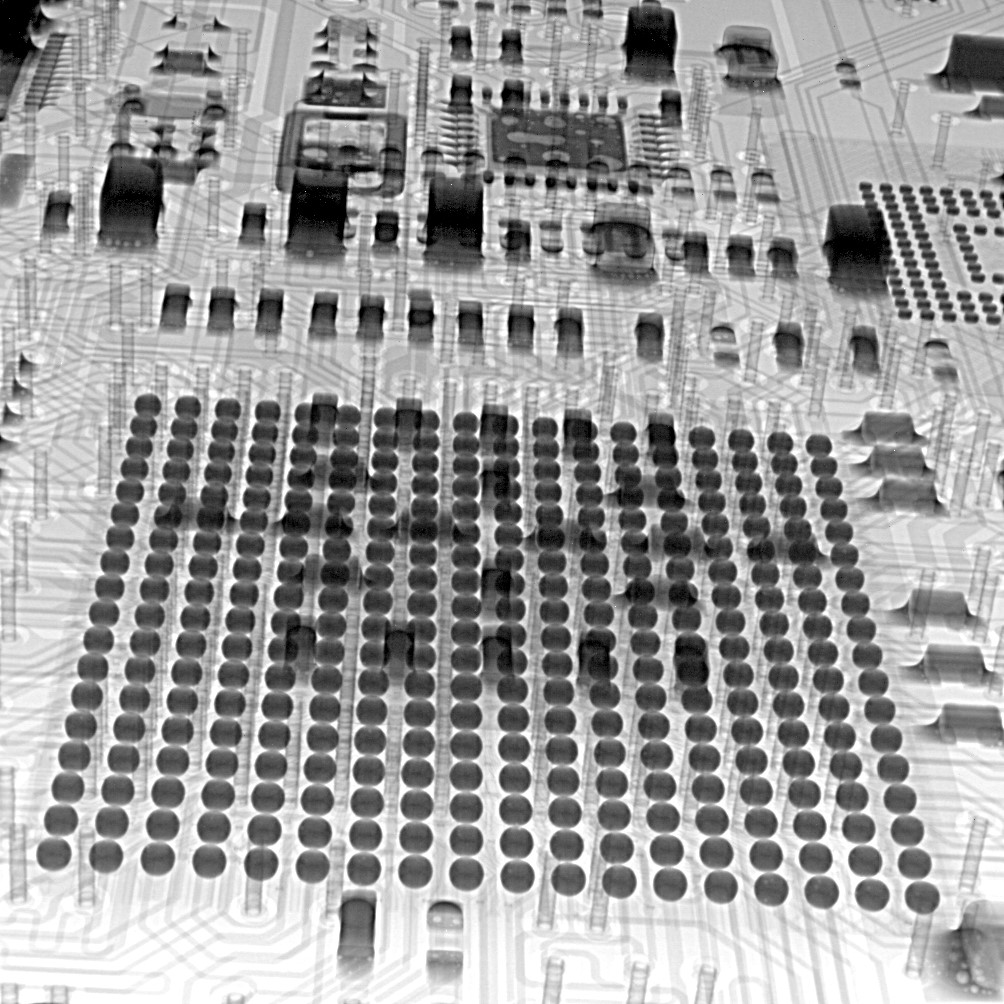
\includegraphics[angle=0,height=10cm]{images/Roentgenbild_U5_2.jpg}
\caption{Röntgenbild vom Prozessor}
\label{fig:roentgenbildProzessor}
\end{figure}


